\chapter{Introduction}

In the following sections, we introduce the key concepts relevant to our research. Since topics such as containerization and container orchestration — and operations in general — are often underrepresented in the academic curriculum, we find it essential to provide the reader with foundational context.

Chapter~\ref{chap:research} forms the core of the theoretical part of our research. It describes the methods employed, the experimental environment we created, and the rationale behind the selection of the tools used.

Chapter~\ref{chap:implementation} focuses on the implementation of the security tool developed as a result of our research. This chapter takes a practical perspective and highlights the most significant engineering aspects of our solution.

Finally, Chapter~\ref{chap:results} summarizes our findings, concludes the research, and reflects on the outcomes achieved through the development of our custom security tool.

\section{Containerization}

When talking about the Kubernetes it is essential to be familiar with the technology of containerization. This chapter introduces the reader to the basics of the containerization. We start by giving a short definition, then we examine core concepts of the containerization such as container image and Docker. Then we compare it to the traditional means of application deployment. Finally, we examine the security on the container image level.

\subsection{Overview}

According to IBM, containerization is the packaging of software code with just the operating system libraries and dependencies required to run the code to create a single lightweight executable—called a container—that runs consistently on any infrastructure. \cite{ibm-containerization}.

Although containers are built to be infrastructure-agnostic, there are still certain compatibility considerations to keep in mind. One significant factor is processor architecture. Containers built for a specific architecture family (e.g., arm64, amd64, or x86) are generally not cross-compatible with infrastructures based on different architectures. However, it is possible to build multi-architecture containers that support multiple processor architectures in a single image, enhancing the flexibility and portability of the containerized applications across diverse environments.

\subsection{Container Image}

Container images are software application packages, which are shipped with all required libraries, binaries and configurations. In another words, container images are lightweight and higly portable artifacts. Usually container images are stored in Container Registries, either public (e.g. Dockerhub) or private. When an image transitions into the running state, it becomes a container.

Container images are comprised of multiple layers. At the base layer there is usually some lightweight Linux distribution. Then, each layer introduce a change in the environment, a change might be in the code or binary, runtimes, dependencies, and other filesystem objects required to run an application.

\subsection{Docker}

Docker is the most widely used containerization tool. It ships tools to build, run and store containers. Docker Engine is a collective name for the Docker build toolkit. First, there is a \lstinline{dockerd} or Docker Daemon, which is a server running in the backend. Secondly, the user intercts with Docker CLI or Docker Client to build and run images. Docker Clients communicates with Docker Daemon through the Rest API served at the backend. Then, there is Docker Compose, which a simple orchestration tool for the containers. It can be used to compose a few containers into a system with a shared network and storage. Lastly, Dockerhub is a public container registry, where the bulk of the publicly available images are stored.

Images are built based on the Dockerfile, which is a set of instructions. Each instruction introduces a new layer to the image. Layers can then be smartly reused by the Docker Engine to build different images with similar bases. Listing~\ref{lst:dockerfile} demonstates an example of the Dockerfile. Each Dockerfile starts with a \lstinline{FROM} command, which specifies the base image to use for this container. The \lstinline{FROM} keyword is followed by the base image name. In our case, \lstinline{registry.redhat.io} is the registry address. It is followed by the repository name (\lstinline{ubi8} in our case), which is separated from the registry name by a single slash and may be preceeded by the namespace. Lastly, tag follows repository name and separated with a colon from it. Both registry address and tag are optional. In case registry name is omitted, Docker will search for the image in the Dockerhub. If the tag is not provided, Docker will fetch \lstinline{latest} tag.

\begin{lstlisting}[language=Dockerfile, caption={A simple Dockerfile for a NodeJS app.}, label={lst:dockerfile}]
    FROM registry.redhat.io/ubi8:latest
    RUN dnf install nodejs && \
        useradd -u 1000 -g 1000 -M node
    COPY --chown=node:node src /app
    WORKDIR /app/src
    USER node
    RUN npm ci
    EXPOSE 3000
    ENTRYPOINT ["npm", "run"]
\end{lstlisting}

\lstinline{RUN} command is used to run commands inside the container during the build phase. All artefacts generated by the \lstinline{RUN} command stay inside the contaier and can be used during runtime. In our case we are installing the necessary binaries to run our application and creating a user to run the application. \lstinline{COPY} command copies the specified resource from the local machine into the container. We also are changing the ownership for the copied files. \lstinline{WORKDIR} command affects the commands after it, so that they are executed from the specified directory. \lstinline{USER} command changes the current user. Last \lstinline{USER} command inside the Dockerfile determines under which user the main process inside the container is running in the runtime. In our case we use our newly created \lstinline{node} user. The default user for the container is \lstinline{root}. \lstinline{EXPOSE} command ensures that a specific port on the container is open for the external communication. Lastly, \lstinline{ENTRYPOINT} is one of the few ways to define the main process of the container. When main process ends, the container stops.

\subsection{Containerization vs Virtualization}

Let us discuss why containerization is the internationally accepted enterprise solution nowadays and why do software arhitects tend to choose it over traditional virtualization solutions.

Figure~\ref{img:containers-vs-virtual-machines} provides a side-by-side comparison of a Virutal Machine and a Cloud infrastructure, each with three applications deployed. We can see that each application on the container side is missing a "Guest OS" layer. Here lies the main advantage of the containers. Absence of the Guest Operating System provides a lot of advantages, which we discuss further below.

\begin{figure}[!hbt]
	\begin{center}
		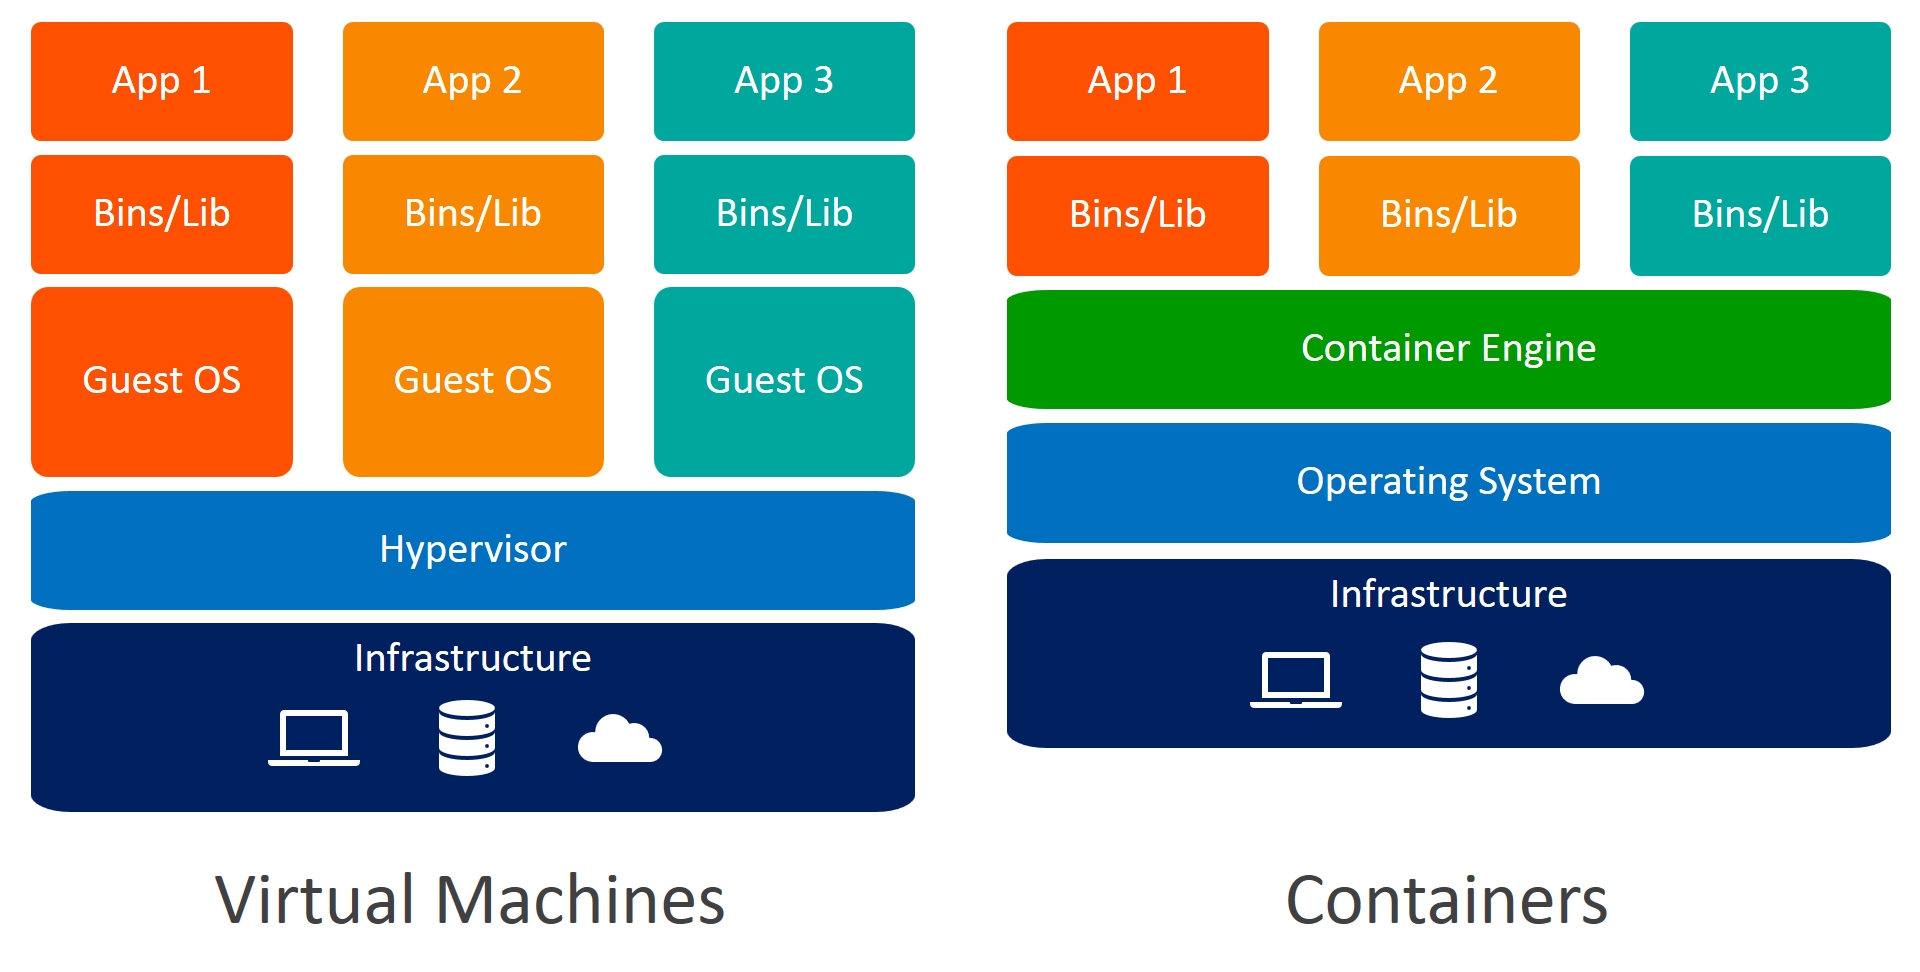
\includegraphics[width=0.75\textwidth]{images/containers-vs-virtual-machines.jpg}
        \caption{Side-by-side comparison of VM and container infrastructures.}
		\label{img:containers-vs-virtual-machines}
	\end{center}
\end{figure}

The most important advantage of the containers is their resource efficiency. Containers only include the application code and its dependencies, which makes them very small compared to the Virtual Machines, which tend to be very bulky and grow in size as development progresses. Containers share the host operating system kernel, so they consume significantly less CPU, memory, and storage than virtual machines, which require a full OS for each instance. This lightweight nature allows more containers to run on a single host, maximizing resource utilization and reducing overhead. Better resource efficiency means also lower costs for the user.

Then, startup speeds are significantly lower for the containers as they do not need to initialize the whole OS boot sequence. This feature also enables the scaling capabilities for the containers, allowing applications to respond quickly to changes in demand.

Additionally, the containers are more consistent than virtual machines. Packed with the required dependencies, they behave in the same way across different environments. As they are isolated from the OS, containers are almost immune to the compatibility issues. This gives them a strong portability advantage. They provide an abstraction that makes it easier to move workloads across various platforms.

Lastly, containers also lead when it comes to automation and CI/CD pipelines. Containers can be easily versioned, updated, and rolled back, allowing for smooth integration into CI/CD pipelines. This streamlines deployment, testing, and rollback processes, leading to faster development cycles. VMs can also be updated and rolled back, but the process is usually slower and more complex.

These are some of the most significant advantages of containerization. All of them contribute to fast build and deploy speeds, which also means high development speeds. While costing less money and providing a lot more flexibility, they become essential for successful enterprise software development. For large-scale development, test and production environment containerization has become an obvious choice over the virtualization.

\subsection{Security Concepts}
\section{Kubernetes}

In this section we will dive into the topic of Kubernetes. We start by shortly overviewing the Kubernetes architecure. Then we expand on the Kubernetes resources, their kinds and their role in the target application environment. Finally, we consider the security of Kubernetes.

\subsection{Overview}

Kubernetes, also known as K8s, is an open source system for automating deployment, scaling, and management of containerized applications. It groups containers that make up an application into logical units for easy management and discovery. Kubernetes builds upon 15 years of experience of running production workloads at Google, combined with best-of-breed ideas and practices from the community. \cite{kubernetes}.

IBM defines Kubernetes as an open source \textbf{container orchestration platform} for scheduling and automating the deployment, management and scaling of containerized applications. Today, Kubernetes and the broader ecosystem of container-related technologies have merged to form the building blocks of modern cloud infrastructure. This ecosystem enables organizations to deliver a highly productive hybrid multicloud computing environment to perform complex tasks surrounding infrastructure and operations. It also supports cloud-native development by enabling a build-once-and-deploy-anywhere approach to building applications. \cite{ibm-kubernetes}.

It is important to emphasize that the Kubernetes abstracts the actual machines (nodes) from the user. Nodes can be physical on-premises servers, or VMs that reside either on-premises or at a cloud provider. Kubernetes takes on the responsibilty of figuring out the deployment target for a particular application. That is, user only defines the desired state of the infrastructure using YAML or JSON configuration files. Kubernetes then creates all the workloads based on the applied configuration.

\subsection{Kubernetes Architecture}

While Kubernetes requires at least three nodes to run, there are some implementation designed for the local use, which emulate this concept (see Subsection~\ref{sec:other-kubernetes-implementations}). The master node is called control plane. The control plane manages the worker nodes and the Pods in the cluster. In production environments, the control plane usually runs across multiple computers and a cluster usually runs multiple nodes, providing fault-tolerance and high availability. Worker nodes host the actual workload inside the cluster. Figure~\ref{img:kubernetes-architecture} provides a simple high-level overview of a typical Kubernetes cluster with a Control Plane and three worker nodes.

\begin{figure}[!hbt]
	\begin{center}
		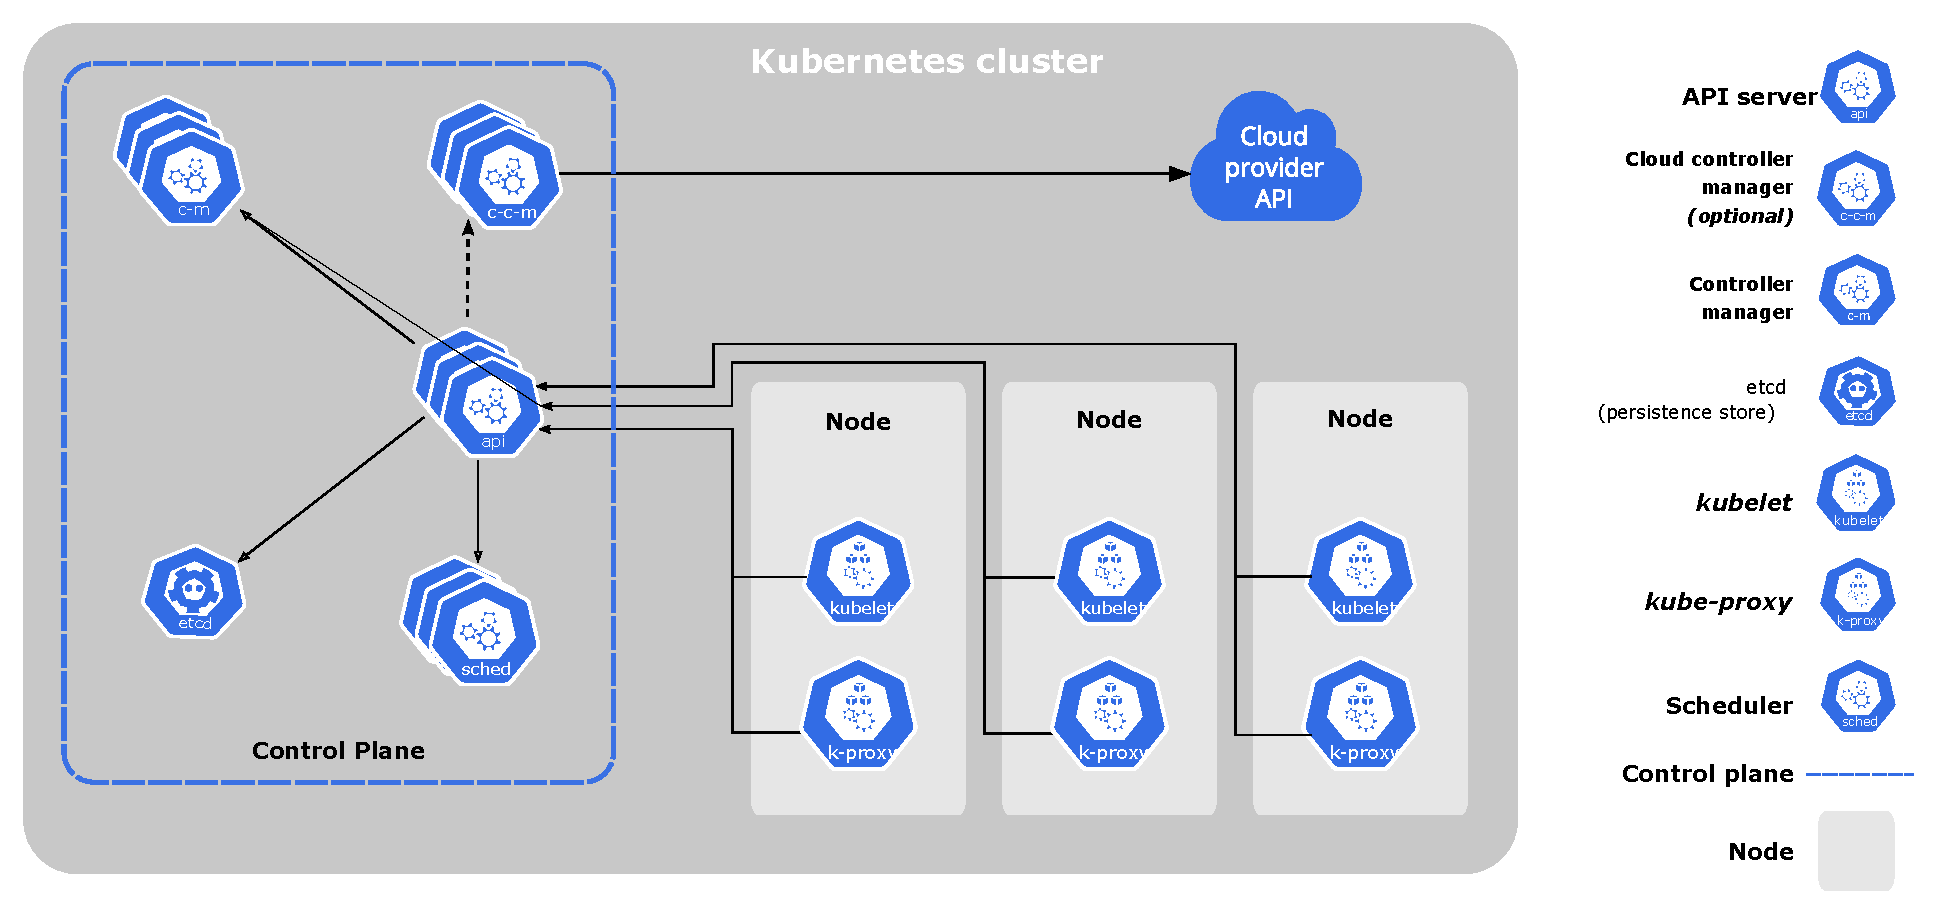
\includegraphics[width=0.85\textwidth]{images/components-of-kubernetes.pdf}
        \caption{Kubernetes cluster architecure overview with its main components.}
		\label{img:kubernetes-architecture}
	\end{center}
\end{figure}

\subsubsection*{Control Plane overview}

Control plane runs the following components: 
\begin{itemize}
\item \textbf{kube-apiserver} \\
Kube-apiserver exposes the Kubernetes API, which is acting as a frontend for the Kubernetes control plane.
\item \textbf{etcd} \\
Etcd is a key-value store, where all of the cluster data is stored.
\item \textbf{kube-scheduler} \\
Each time a new pod is created, it is passed to the kube-scheduler, which assigns the pod to the specific node to run on (based on individual and collective resource requirements, hardware/software/policy constraints, affinity and anti-affinity specifications, data locality, inter-workload interference, and deadlines).
\item \textbf{kube-controller-manager} \\
Each Kubernetes resource has its own controller (e.g. NodeController, JobController, ServiceAccountController); all of them are compiled as one binary called kube-controller-manager.
\item \textbf{cloud-controller-manager} \\
Cloud-controller-manager embeds cloud-specific control logic. It differs depending on the cloud provider or can be absent completely, when running Kubernetes locally.
\end{itemize}

\subsubsection*{Worker Node overview}

Each worker node has a kubelet and kube-proxy installed. Kubelet is an agent that manages runnning pods and containers. Kube-proxy is a network proxy that implements parts of the Kubernetes service concept. It maintains network rules on nodes, making in- outside-cluster communitcation possible.

Then, of course, each worker node has a set of running pods. A typical use would involve multiple running applications. Depending on the size of the node and the application resoucre consumption it can accomodate on average from one to a few dozens applications with various business purposes.

\subsection{Kubernetes Resources}

Kubernetes resources are fundamental components that define various entities within a Kubernetes cluster. Resources are objects that represent the desired state and configuration of the infrastructure, applications, and services running on the cluster. Kubernetes provides a range of resources that enable developers and operators to define, manage, and scale containerized applications, network policies, storage requirements, and more. These resources are defined declaratively in YAML or JSON files, which makes infrastructure setup consistent and reproducible.

Among key Kubernetes resoucres are:
\begin{itemize}
    \item \textbf{Pods} \\
        Pod is the atomic workload unit in the Kubernetes cluster. It encapsulates one or more containers that share the same network. It represents a single instance of a running application.
    \item \textbf{Deployments} \\
        Deployments are a higher level of abstraction for the Pods. They allow to define replica count and rollout/rollback strategy for the updates, which can be used to ensure availability for the application.
    \item \textbf{Services} \\
        Services provide a communication layer for the pods inside one cluster. Being an abstraction over the pods' network, they provide reliable access to the selected workloads, while serving as a Load Balancer. 
    \item \textbf{ConfigMaps} and \textbf{Secrets} \\
        ConfigMaps and Secrets allow users to store data outside the workload. ConfigMaps are usually used to store non-sensitive information like environment and application configuration parameters. Secrets are a more secure resource designed for API keys, passwords and other sensitive data.
    \item \textbf{PersistentVolumes} and \textbf{PersistentVolumeClaims} \\
        These resources enable stateful applications to request and mount durable storage within a cluster, allowing data to persist independently of the Pod lifecycle.
\end{itemize}

Above are the most commonly used resources, which we also leverage in the practical part of the paper. Therefore, it is important that the reader understands the position and the purpose of each resource in the cluster infrastructure.

\subsubsection*{Workloads}

Minimal computing units in Kubernetes are Containers, which are running in Pods. However, to simplify the management of Pods, Kubernetes has workload resources, which manage the set of Pods. They make sure the desired number of Pods of right kind are running to match the declaration.

Deployments and ReplicaSets are a good fit for stateless applications. Each pod in the Deployment is interchangebeable. Deployments are easily scalable and have built-in versioning and rollout mechanisms.

StatefulSet allows to create sets of stateful applications. They might share the same PersistentVolume and replicate data between each other.

DaemonSet defines Pods that provide node-local facilities. These might be fundamental to the operation of your cluster, such as a networking helper tool, or be part of an add-on.

Job and CronJob define tasks that run to completion and then stop. Jobs represent one-off tasks, whereas CronJobs recur according to a schedule.

\subsubsection*{Networking}

Kubernetes networking model makes Pods look like VMs in the networking aspect. Pods on any nodes can communicate with each other without NAT. Containers inside the same Pod share its network meaning that they can reach each other using localhost.

Kubernetes networking addresses four concerns:
\begin{itemize}
\item Containers within a Pod use networking to communicate via loopback.
\item Cluster networking provides communication between different Pods.
\item The Service API lets you expose an application running in Pods to be reachable from outside your cluster.
\item Ingress provides extra functionality specifically for exposing HTTP applications, websites and APIs.
\item You can also use Services to publish services only for consumption inside your cluster.
\end{itemize}

\subsubsection*{Storage}

Kubernetes does not ship a particular implementation of storage. However, it provides a range of resources that define the storage concept and supports different types of volumes. A Pod can use any number of volume types simultaneously. Ephemeral volume types have a lifetime of a pod, but persistent volumes exist beyond the lifetime of a pod. When a pod ceases to exist, Kubernetes destroys ephemeral volumes; however, Kubernetes does not destroy persistent volumes. For any kind of volume in a given pod, data is preserved across container restarts.

At its core, a volume is a directory, possibly with some data in it, which is accessible to the containers in a pod. How that directory comes to be, the medium that backs it, and the contents of it are determined by the particular volume type used.

PersistentVolumes and PersistentVolumeClaims are the resources kinds most important to understand here.
\begin{itemize}
\item A PersistentVolume (PV) is a piece of storage in the cluster that has been provisioned by an administrator or dynamically provisioned using Storage Classes. It is a resource in the cluster just like a node is a cluster resource. PVs are volume plugins like Volumes, but have a lifecycle independent of any individual Pod that uses the PV. This API object captures the details of the implementation of the storage, be that NFS, iSCSI, or a cloud-provider-specific storage system.
\item A PersistentVolumeClaim (PVC) is a request for storage by a user. It is similar to a Pod. Pods consume node resources and PVCs consume PV resources. Pods can request specific levels of resources (CPU and Memory). Claims can request specific size and access modes (e.g., they can be mounted ReadWriteOnce, ReadOnlyMany or ReadWriteMany). Once and Many here refer to a number of Pods that can perform the read or write simultaneously.
\end{itemize}

\subsection{Infrastructure Security}

When we are talking about the infrastructure security, we must consider multiple layers. Going from the top to the bottom, we start with the security measurements taken on the Cloud provider side. In most cases this is not something we can affect and the security of different Cloud providers varies significantly. Unfortunately, this is out of scope of this paper, but all of the "big five" Cloud providers (AWS, Azure, Google Cloud, Alibaba and IBM) maintain high security standarts and security risks generally should not be a concern for their end users. Then, we get to the cluster itself. On the cluster level we must consider the security of the nodes, security of the cluster components and their configuration. At this layer we have already some space for the misconfigurations to appear. Here we can evaluate the security of the single components using some of the security scanners presented in \nameref{sec:kubernetes-security-automation}. Lastly, we get to the application level, where the security of the application code, Kubernetes resoucre configuration, libraries, dependencies and base images is the main concern. Again, this is the layer, where the developers have the most access to, thus, providing a lot of space for the possibility of a human error. In this paper we mostly work on this level when we do our research.

Officially, The Linux Foundation provides only some security guidelines for each of the layers. However, bundled with Kubernetes we get a few means to keep the security under control. Below we present an overview of the Kubernetes security recommendations, RBAC and Data security inside Kubernetes.

\subsubsection*{Kubernetes security recommendations}

This section gathers the official security recommendations provided by the Kubernetes. They provide a list of concerns for each level of the cloud infrastructure. Cloud infrastructure can be viewed as a composition of four layers as displayed by the Figure~\ref{img:cloud-security}.

\begin{figure}[!hbt]
	\begin{center}
		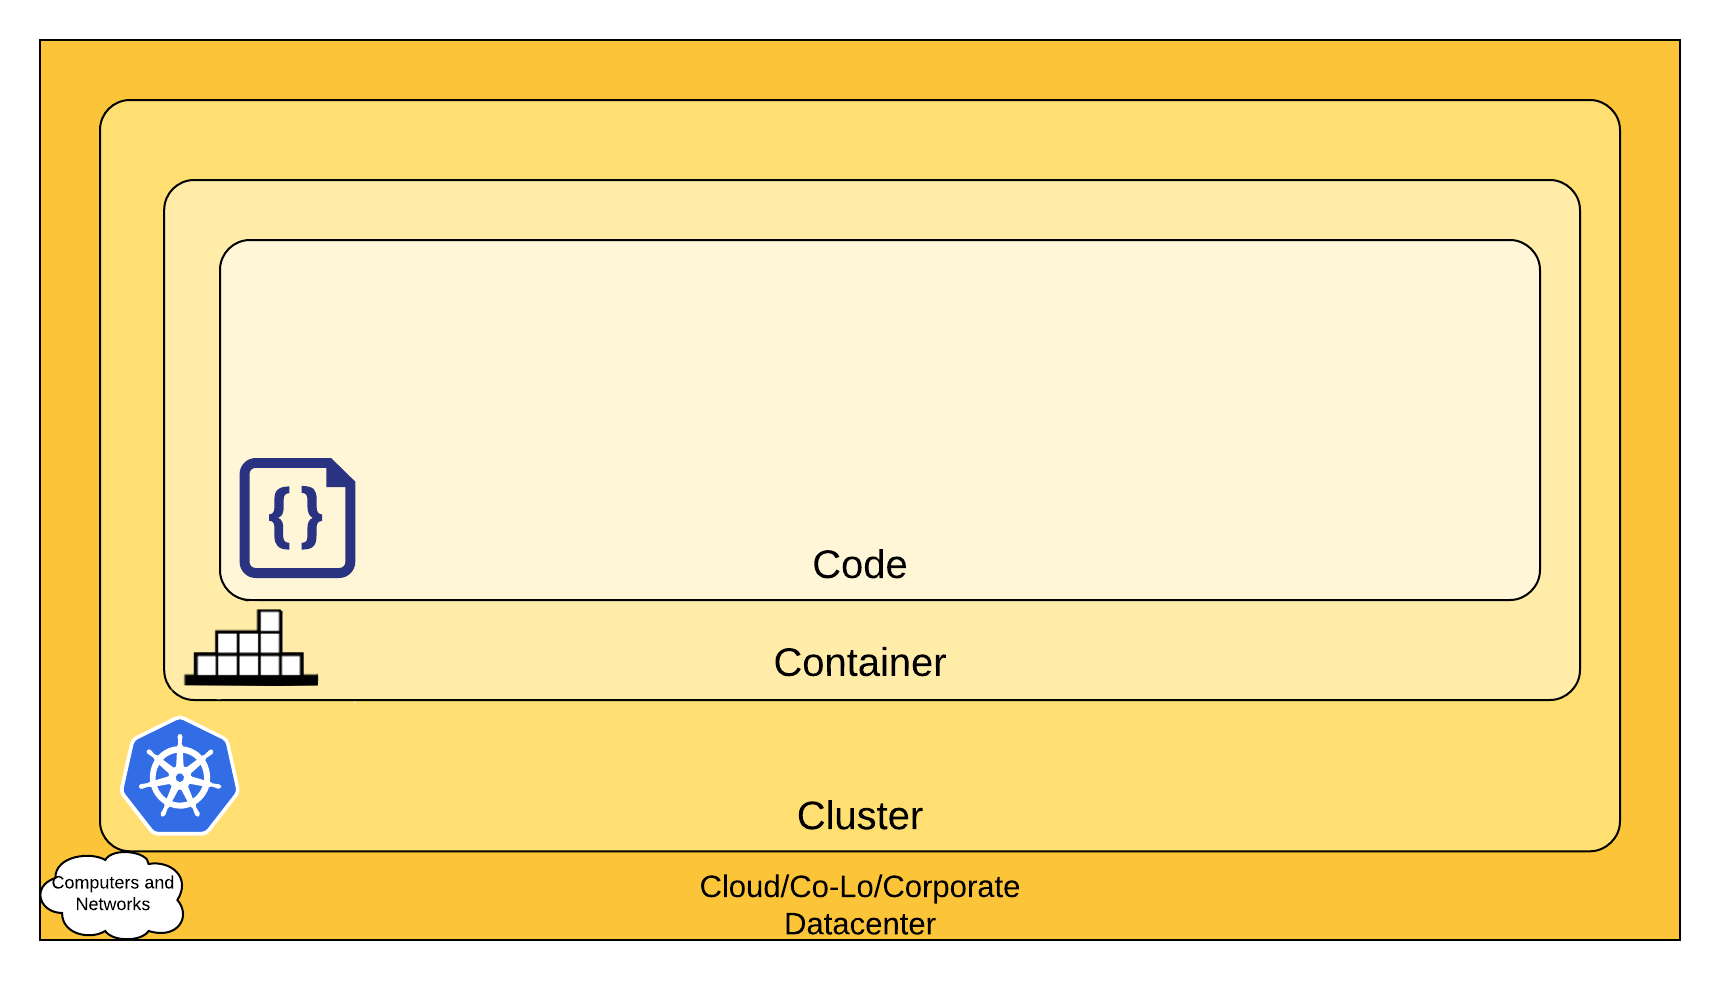
\includegraphics[width=0.75\textwidth]{images/cloud-security.png}
        \caption{Four layers of the cloud infrastructure.}
		\label{img:cloud-security}
	\end{center}
\end{figure}

Each layer is built upon the previous one and its security depends on the security of the outer layers. It is, therefore, important to maintain high security standarts on base levels (Cloud, Cluster, Container).

\begin{enumerate}

\item \textbf{Cloud} \\
Each cloud provider has its own security policies and guidelines. There are, however, some general infrastructure-level security best advice described by in the Table~\ref{tab:cloud-security-recommendations}.

\begin{table}[H]
    \begin{center}
        \begin{tabular}{ | p{.20\textwidth} | p{.80\textwidth} | } 
         \hline
         \textbf{Area of Concern for Kubernetes Infrastructure} & \textbf{Recommendation} \\ 
         \hline
         Network access to API Server (Control plane) & All access to the Kubernetes control plane is not allowed publicly on the internet and is controlled by network access control lists restricted to the set of IP addresses needed to administer the cluster. \\ 
         \hline
         Network access to Nodes (nodes)  & Nodes should be configured to only accept connections (via network access control lists) from the control plane on the specified ports, and accept connections for services in Kubernetes of type NodePort and LoadBalancer. If possible, these nodes should not be exposed on the public internet entirely. \\ 
         \hline
         Kubernetes access to Cloud Provider API & Each cloud provider needs to grant a different set of permissions to the Kubernetes control plane and nodes. It is best to provide the cluster with cloud provider access that follows the principle of least privilege for the resources it needs to administer. \\
         \hline
         Access to etcd & Access to etcd (the datastore of Kubernetes) should be limited to the control plane only. Depending on your configuration, you should attempt to use etcd over TLS. \\
         \hline
         etcd Encryption & Wherever possible it's a good practice to encrypt all storage at rest, and since etcd holds the state of the entire cluster (including Secrets) its disk should especially be encrypted at rest. \\
         \hline
        \end{tabular}
    \end{center}
    \caption{Security recommendations for the Cloud layer.}
    \label{tab:cloud-security-recommendations}
\end{table}

\item \textbf{Cluster} \\
There are two cluster security concerns that could be addressed: securing the configurable cluster components and securing the applications running in the cluster.

There are a few things to consider regarding the application security:
\begin{itemize}
\item RBAC Authorization (Access to the Kubernetes API)
\item Authentication	
\item Application secrets management (and encrypting them in etcd at rest)
\item Ensuring that pods meet defined Pod Security Standards
\item Quality of Service (and Cluster resource management)
\item Network Policies
\item TLS for Kubernetes Ingress
\end{itemize}

\item \textbf{Container} \\
Securing containers is a vast topic, which deserves its own chapter. There are, nevertheless, a few general recommendation provided by the Kubernetes, which you can find in the Table~\ref{tab:container-security-recommendations}.

\begin{table}[H]
    \begin{center}
        \begin{tabular}{ | p{.20\textwidth} | p{.80\textwidth} | } 
        \hline
        \textbf{Area of Concern for Containers} & \textbf{Recommendation} \\ 
        \hline
        Container Vulnerability Scanning and OS Dependency Security & As part of an image build step, you should scan your containers for known vulnerabilities. \\ 
        \hline
        Image Signing and Enforcement & Sign container images to maintain a system of trust for the content of your containers. \\ 
        \hline
        Disallow privileged users & When constructing containers, create users inside of the containers that have the least level of operating system privilege necessary in order to carry out the goal of the container. \\
        \hline
        \end{tabular}
    \end{center}
    \caption{Security recommendations for the Container layer.}
    \label{tab:container-security-recommendations}
\end{table}

\item \textbf{Code} \\
When it comes to code, the developers have the most flexibility to design secure applications. There are a lot of issues to address, which may vary significantly from application to application depending on its purpose, architecture and framework base. Kubernetes documentation gives a handful of recommendations regarding this topic, which are displayed below in the Table~\ref{tab:code-security-recommendations}.

\begin{table}[H]
    \begin{center}
        \begin{tabular}{ | p{.20\textwidth} | p{.80\textwidth} | } 
        \hline
        \textbf{Area of Concern for Code} & \textbf{Recommendation} \\ 
        \hline
        Access over TLS only & If your code needs to communicate by TCP, perform a TLS handshake with the client ahead of time. With the exception of a few cases, encrypt everything in transit. Going one step further, it's a good idea to encrypt network traffic between services. This can be done through a process known as mutual TLS authentication or mTLS which performs a two sided verification of communication between two certificate holding services. \\ 
        \hline
        Limiting port ranges of communication & This recommendation may be a bit self-explanatory, but wherever possible you should only expose the ports on your service that are absolutely essential for communication or metric gathering. \\ 
        \hline
        3rd Party Dependency Security & It is a good practice to regularly scan your application's third party libraries for known security vulnerabilities. Each programming language has a tool for performing this check automatically. \\
        \hline
        Static Code Analysis & Most languages provide a way for a snippet of code to be analyzed for any potentially unsafe coding practices. Whenever possible you should perform checks using automated tooling that can scan codebases for common security errors. \\
        \hline
        Dynamic probing attacks & There are a few automated tools that you can run against your service to try some of the well known service attacks. These include SQL injection, CSRF, and XSS. One of the most popular dynamic analysis tools is the OWASP Zed Attack proxy tool. \\
        \hline
        \end{tabular}
    \end{center}
    \caption{Security recommendations for the Code layer.}
    \label{tab:code-security-recommendations}
\end{table}
                      
\end{enumerate}

\subsubsection*{Role Based Access Control}

\subsubsection*{Data security}

\subsection{Other Kubernetes Implementations}
\label{sec:other-kubernetes-implementations}

\subsubsection*{Openshift}

\subsubsection*{Rancher Desktop}
\section{Security frameworks}

\subsection{Overview}

When we are talking about the infrastructure security of Kuberntes environment inside the cloud, we must consider multiple layers. Going from the top to the bottom, we start with the security measurements taken on the cloud provider side. In most cases this is not something we can affect and the security of different cloud providers varies significantly. However, all of the ``big five'' cloud providers (AWS, Azure, Google Cloud, Alibaba and IBM) maintain high security standarts and security risks generally should not be a concern for their end users. Then, we get to the cluster itself. On the cluster level we must consider the security of the nodes, security of the cluster components and their configuration. At this layer we have already some space for the misconfigurations to appear. Here we can evaluate the security of the single components using some of the security scanners presented in \nameref{sec:kubernetes-security-automation}. But it should be noted that the cluster can only be as secured as its nodes. Therefore, attention should be given to the node security first. Host operating system should be regularly patched with the most recent security patches. Lastly, we get to the application level, where the security of the application code, Kubernetes resoucre configuration, libraries, dependencies and base images is the main concern. Again, this is the layer, where the developers have the most access to, thus, providing a lot of space for the possibility of a human error. In this paper we mostly work on this level when we do our research.

Over the years a variety of Kubernetes security frameworks have been developed. There are a few that target specific layers of the Kubernetes environment, but most of them are designed to assess the security on a combination of those layers. In the Kubernetes scope, security framework is a structured set of guidelines and policies designed to assess, implement and maintain security controls across different Kuberntes layers. Kubernetes security frameworks are modular (as they are usually split across different domains) and provide guidelines to minimize risks or remediation instructions to resolve the threat. Among the most well-known Kubernetes security frameworks are CIS Kubernetes Benchmark, NSA Framework and MITRE ATT\&CK Framework. Among other notable frameworks are NIST 800-53 and SOC 2. The former is a comprehensive security and privacy control framework developed by the National Institute of Standards and Technology. The latter is a compliance framework designed by the AICPA, which focuses on how companies manage customer data. Payment card data security is considered by the PCI-DSS framework and the clusters used for processing card data must comply. GDPR also applies to the Kubernetes deployments if they process personal data of EU citizens. HIPAA is a framework that regulates the privacy and security of health information. Clusters hosting applications that handle ePHI must enforce encryption, logging, access control, and backup policies. ISO/IEC 27001 is an international standard for establishing, implementing, maintaining, and continuously improving an Information Security Management System, which can be applied to the Kubernetes as well.

Officially, The Kubernetes project itself (and CNCF) publish some security guidelines for each of the layers. However, a more thourough and complete list of Kubernetes security checks are provided by the Center of Internet Security, National Security Agency and MITRE Corporation. Below we present an overview of the Kubernetes security recommendations by CNCF, and an overview of the most popular security frameworks.

\subsection{Kubernetes security recommendations}

This section gathers the official security recommendations provided by the Kubernetes. They provide a list of concerns for each level of the cloud infrastructure. Cloud infrastructure can be viewed as a composition of four layers as displayed by the Fig~\ref{img:cloud-security}.

\begin{figure}[!hbt]
	\begin{center}
		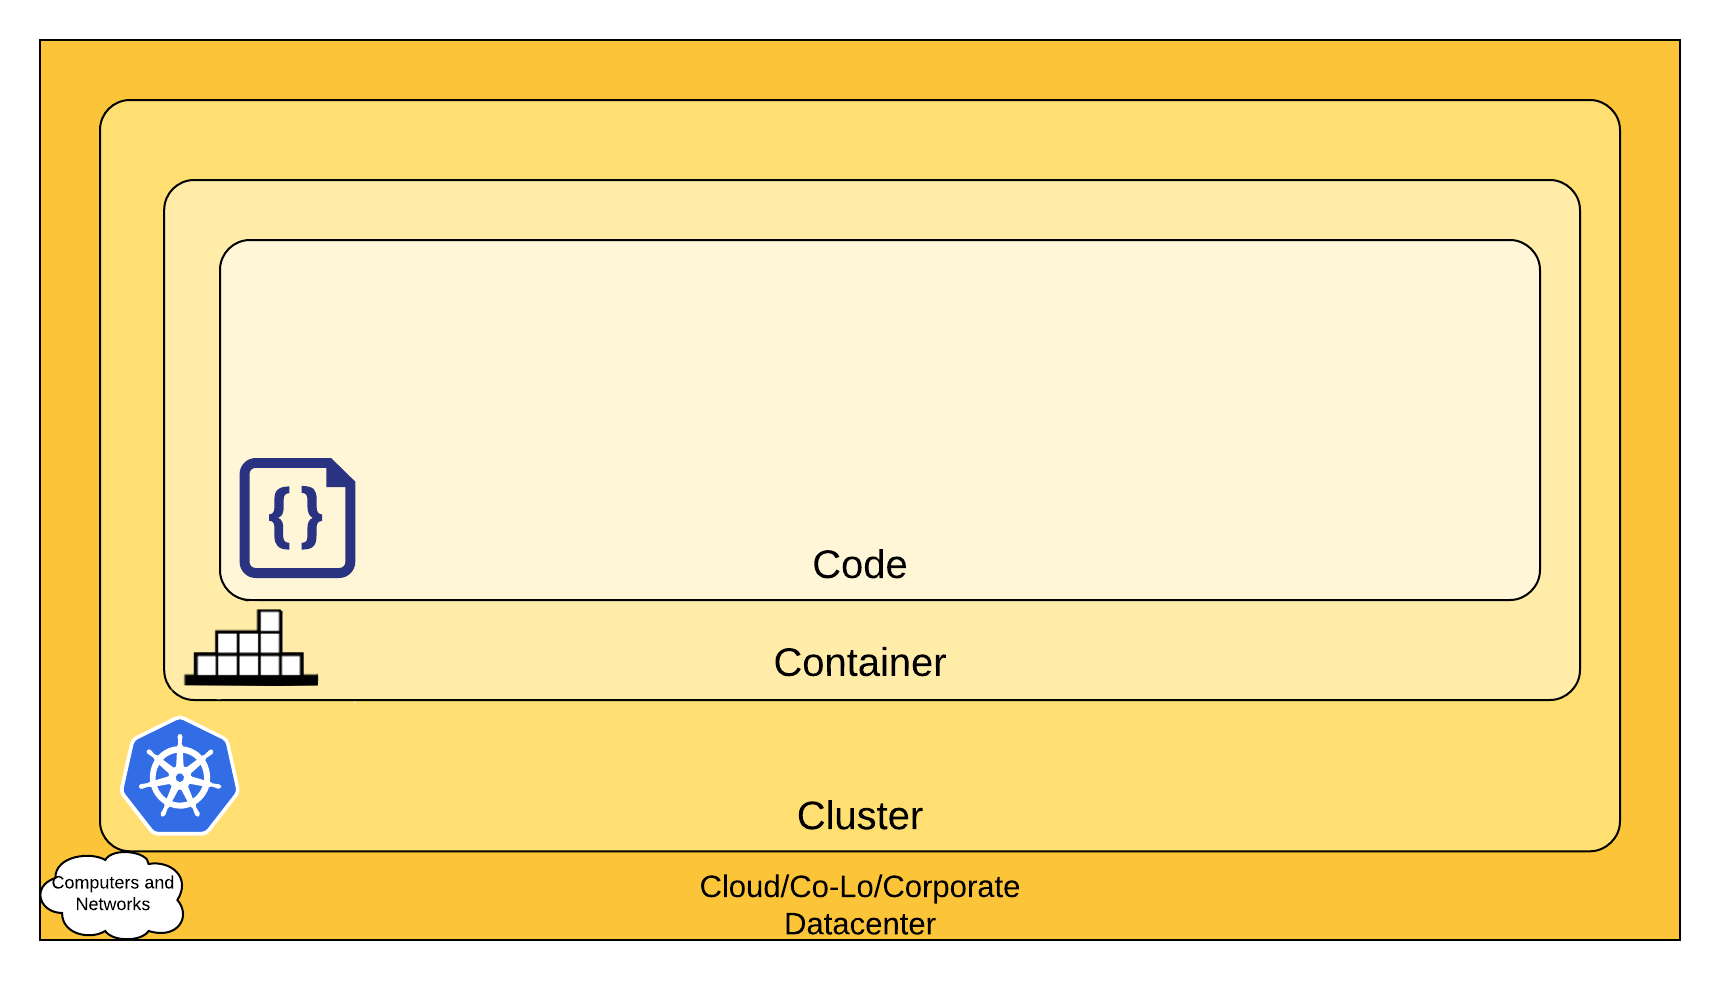
\includegraphics[width=0.75\textwidth]{images/cloud-security.png}
        \caption{Four layers of the cloud infrastructure.}
		\label{img:cloud-security}
	\end{center}
\end{figure}

Each layer is built upon the previous one and its security depends on the security of the outer layers. It is, therefore, important to maintain high security standarts on base levels (cloud, cluster, container).

\begin{enumerate}

\item \textbf{Cloud} \\
Each cloud provider has its own security policies and guidelines. There are, however, some general infrastructure-level security best advice described by in the Tab~\ref{tab:cloud-security-recommendations}.

\begin{table}[H]
    \begin{center}
        \begin{tabular}{ | >{\raggedright\arraybackslash}p{.20\textwidth} 
                         | >{\raggedright\arraybackslash}p{.75\textwidth} | } 
         \hline
         \textbf{Area of Concern for Kubernetes Infrastructure} & \textbf{Recommendation} \\ 
         \hline
         Network access to API Server (Control plane) & All access to the Kubernetes control plane is not allowed publicly on the internet and is controlled by network access control lists restricted to the set of IP addresses needed to administer the cluster. \\ 
         \hline
         Network access to Nodes (nodes)  & Nodes should be configured to only accept connections (via network access control lists) from the control plane on the specified ports, and accept connections for services in Kubernetes of type NodePort and LoadBalancer. If possible, these nodes should not be exposed on the public internet entirely. \\ 
         \hline
         Kubernetes access to cloud provider API & Each cloud provider needs to grant a different set of permissions to the Kubernetes control plane and nodes. It is best to provide the cluster with cloud provider access that follows the principle of least privilege for the resources it needs to administer. \\
         \hline
         Access to etcd & Access to etcd (the datastore of Kubernetes) should be limited to the control plane only. Depending on your configuration, you should attempt to use etcd over TLS. \\
         \hline
         etcd Encryption & Wherever possible it's a good practice to encrypt all storage at rest, and since etcd holds the state of the entire cluster (including Secrets) its disk should especially be encrypted at rest. \\
         \hline
        \end{tabular}
    \end{center}
    \caption{Security recommendations for the cloud layer.}
    \label{tab:cloud-security-recommendations}
\end{table}

\item \textbf{Cluster} \\
There are two cluster security concerns that could be addressed: securing the configurable cluster components and securing the applications running in the cluster.

There are a few things to consider regarding the application security:
\begin{itemize}
\item RBAC Authorization (Access to the Kubernetes API)
\item Authentication	
\item Application secrets management (and encrypting them in etcd at rest)
\item Ensuring that pods meet defined Pod Security Standards
\item Quality of Service (and Cluster resource management)
\item Network Policies
\item TLS for Kubernetes Ingress
\end{itemize}

\item \textbf{Container} \\
Securing containers is a vast topic, which deserves its own chapter. There are, nevertheless, a few general recommendation provided by the Kubernetes, which you can find in the Tab~\ref{tab:container-security-recommendations}.

\begin{table}[H]
    \begin{center}
        \begin{tabular}{ | >{\raggedright\arraybackslash}p{.30\textwidth} 
                         | >{\raggedright\arraybackslash}p{.65\textwidth} | } 
        \hline
        \textbf{Area of Concern for Containers} & \textbf{Recommendation} \\ 
        \hline
        Container Vulnerability Scanning and OS Dependency Security & As part of an image build step, you should scan your containers for known vulnerabilities. \\ 
        \hline
        Image Signing and Enforcement & Sign container images to maintain a system of trust for the content of your containers. \\ 
        \hline
        Disallow privileged users & When constructing containers, create users inside of the containers that have the least level of operating system privilege necessary in order to carry out the goal of the container. \\
        \hline
        \end{tabular}
    \end{center}
    \caption{Security recommendations for the Container layer.}
    \label{tab:container-security-recommendations}
\end{table}

\item \textbf{Code} \\
When it comes to code, the developers have the most flexibility to design secure applications. There are a lot of issues to address, which may vary significantly from application to application depending on its purpose, architecture and framework base. Kubernetes documentation gives a handful of recommendations regarding this topic, which are displayed below in the Tab~\ref{tab:code-security-recommendations}.

\begin{table}[H]
    \begin{center}
        \begin{tabular}{ | >{\raggedright\arraybackslash}p{.20\textwidth} 
                         | >{\raggedright\arraybackslash}p{.75\textwidth} | } 
        \hline
        \textbf{Area of Concern for Code} & \textbf{Recommendation} \\ 
        \hline
        Access over TLS only & If your code needs to communicate by TCP, perform a TLS handshake with the client ahead of time. With the exception of a few cases, encrypt everything in transit. Going one step further, it's a good idea to encrypt network traffic between services. This can be done through a process known as mutual TLS authentication or mTLS which performs a two sided verification of communication between two certificate holding services. \\ 
        \hline
        Limiting port ranges of communication & This recommendation may be a bit self-explanatory, but wherever possible you should only expose the ports on your service that are absolutely essential for communication or metric gathering. \\ 
        \hline
        3rd Party Dependency Security & It is a good practice to regularly scan your application's third party libraries for known security vulnerabilities. Each programming language has a tool for performing this check automatically. \\
        \hline
        Static Code Analysis & Most languages provide a way for a snippet of code to be analyzed for any potentially unsafe coding practices. Whenever possible you should perform checks using automated tooling that can scan codebases for common security errors. \\
        \hline
        Dynamic probing attacks & There are a few automated tools that you can run against your service to try some of the well known service attacks. These include SQL injection, CSRF, and XSS. One of the most popular dynamic analysis tools is the OWASP Zed Attack proxy tool. \\
        \hline
        \end{tabular}
    \end{center}
    \caption{Security recommendations for the Code layer.}
    \label{tab:code-security-recommendations}
\end{table}

\end{enumerate}


\subsection{CIS Kubernetes Benchmark}
\label{sss:cis-kubernetes-benchmark}

CIS publishes a variety of documents for an array of different platforms and infrastructure components. Benchmarks are available for 10 cloud providers, 26 operating systems, 19 kinds of system software, as well as for mobile devices, network devices and desktop software. Benchmarks for the cloud services, for instance, include such cloud providers as Alibaba, Amazon, Google, IBM, Microsoft, Oracle and a few others. For Kubernetes platform, specifically, GKE, AKS, EKS and general Kubernetes benchmarks are available for non-commercial use. 

CIS Benchmark is a PDF file, which contains a list of checks (both manual and automated), that can be performed to ensure the most secure environment. CIS Benchmark file for Kubernetes has 5 categories of security recommendations:
\begin{enumerate}[noitemsep]
    \item Control Plane Components
    \item etcd
    \item Control Plane Configuration
    \item Worker Nodes
    \item Policies
\end{enumerate}

There are multiple subcategories for the most of the categories as well. Each recommendation includes the general information about the check, such as title, description and assessment status. Audit procedure describes the steps necessary to determine if the target system is compliant with the recommendation. Additionaly, every recommendation is supplied with the rationale statement, which gives a ``Detailed reasoning for the recommendation to provide the user a clear and concise understanding on the importance of the recommendation.'' Finally, remediation procedure provides instructions for bringing the the target system into compliance with the recommendation.

CIS Benchmark document \cite{cis-kubernetes-benchmark} states that ```All CIS Benchmarks (Benchmarks) focus on technical configuration settings used to maintain and/or increase the security of the addressed technology, and they should be used in conjunction with other essential cyber hygiene tasks ... In the end, the Benchmarks are designed to be a key component of a comprehensive cybersecurity program.''' This means that even though benchmarks cover many aspects of Kubernetes security, authors recommend to use in combination with other defensinve and monitoring tools.

\subsection{NSA Framework}

The NSA Kubernetes Hardening Guide is a security framework jointly published by the U.S. National Security Agency and CISA. It provides actionable recommendations to secure Kubernetes clusters against real-world threats. As stated in the document itself \cite{nsa-kubernetes-hardening-guide}, it ``describes the security challenges associated with setting up and securing a Kubernetes cluster. It includes strategies for system administrators and developers of National Security Systems, helping them avoid common misconfigurations and implement recommended hardening measures and mitigations when deploying Kubernetes''. First released in August 2021, it was last updated in August 2022, but is still used worldwide as the most of the described concepts are still applicable to the newest Kubernetes versions.

This guide is a well-structured document 66 pages long. It is written as a text guide and divided into multiple sections. The sections are Kubernetes Pod Security, Network Separation and Hardening, Authentication and Authorization, Audit Logging and Threat Detection, Upgrading and Application Security Practices. Each section describes the best security practices for a particular domain. For instance, the document proposes a hardened container build workflow, where each image must pass three security services (image signature verification, image scanner, configuration validation) before being deployed into the cluster. Figure~\ref{img:hardened-container-build-workflow} displays a schematic overview of the workflow. Interstingly, the document references and is partially based on MITRE ATT\&CK Framework.

\begin{figure}[!hbt]
	\begin{center}
		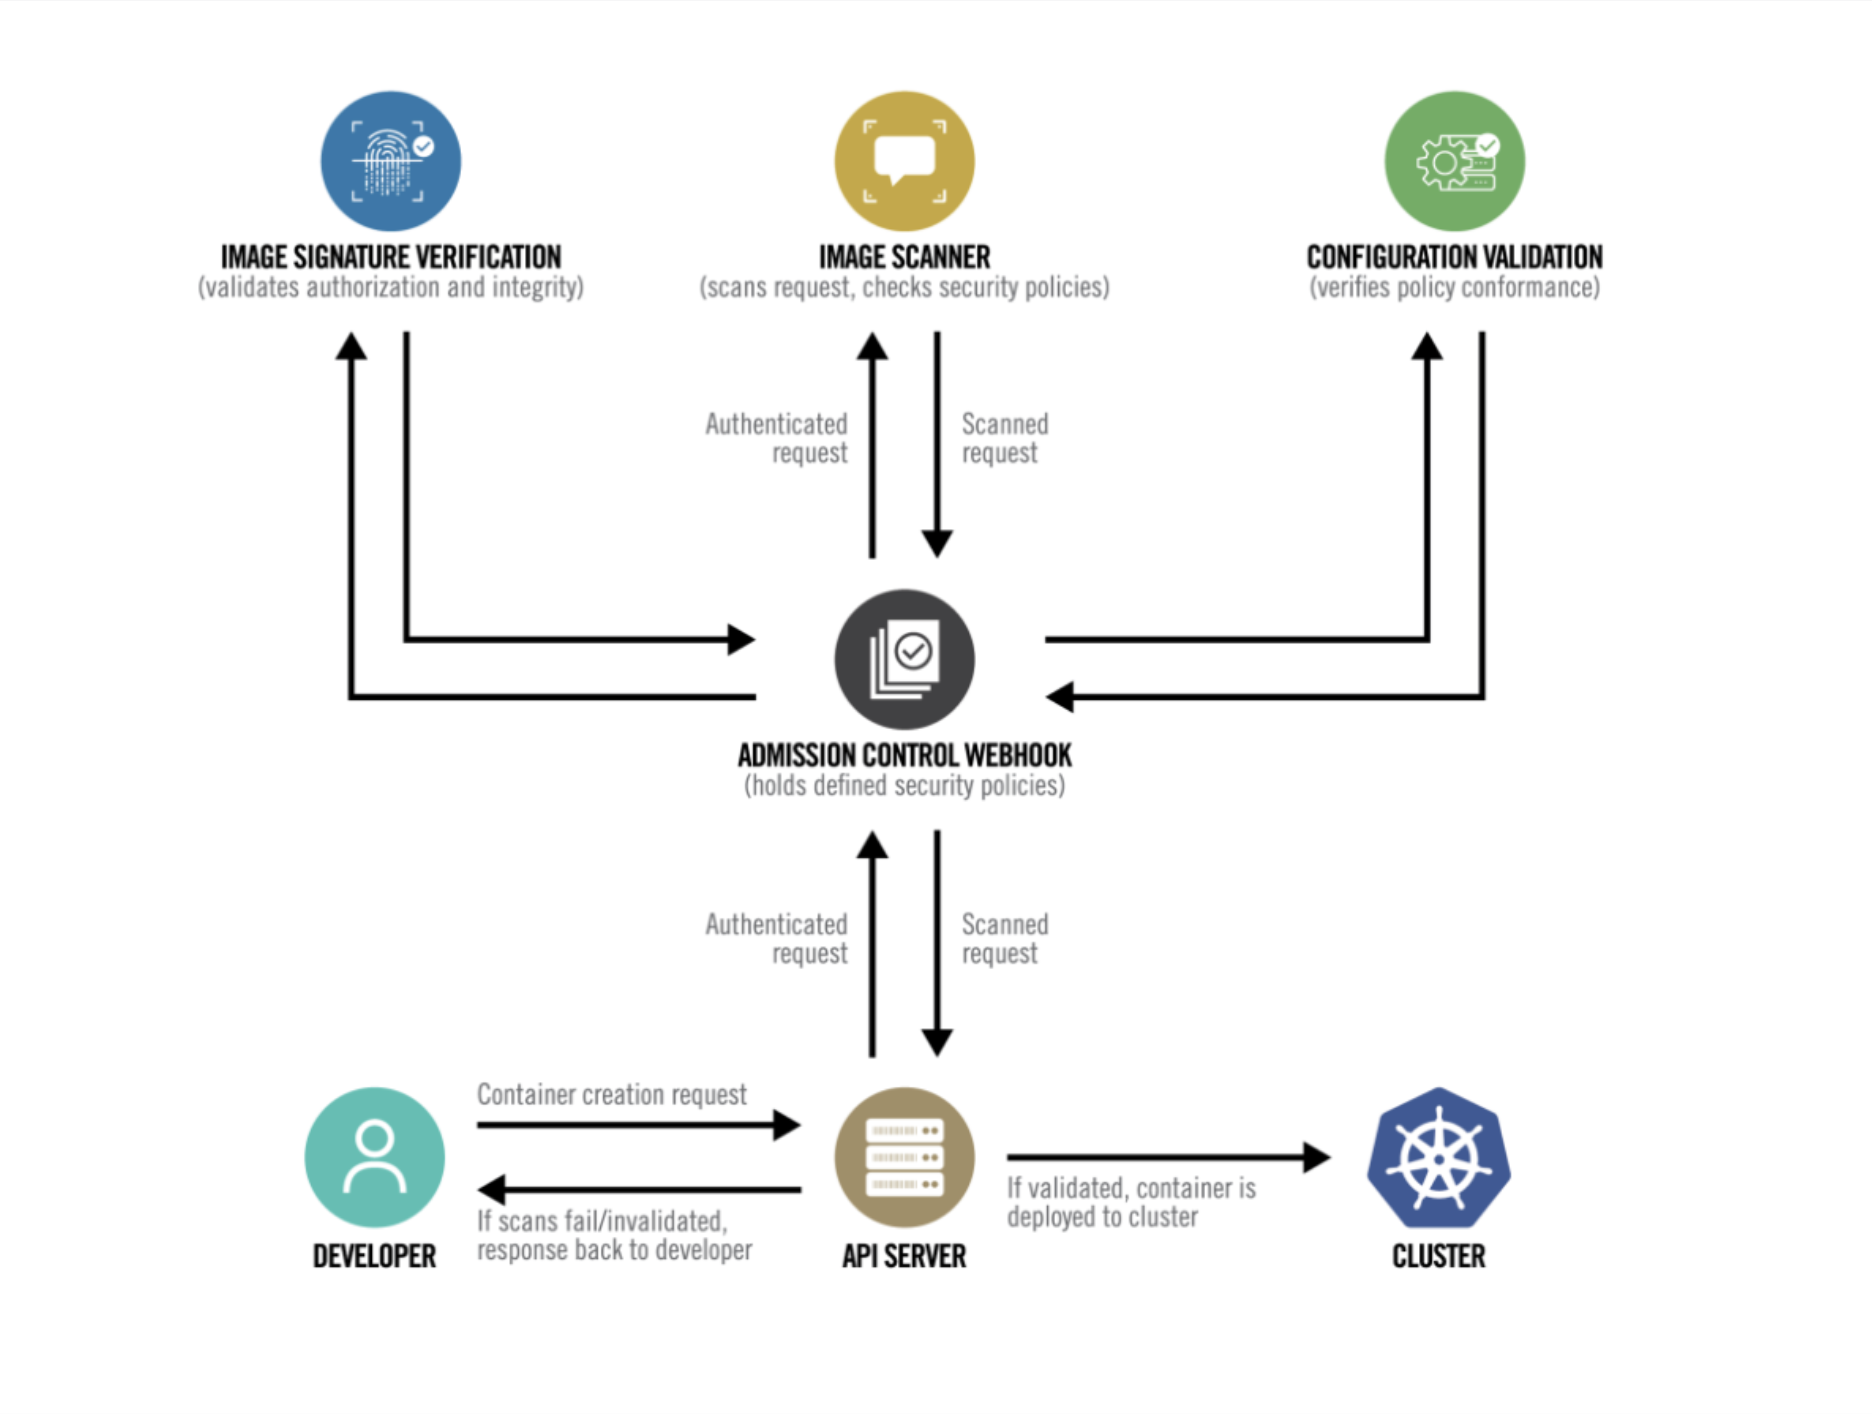
\includegraphics[width=0.9\textwidth]{images/hardened-container-build-workflow.png}
        \caption{A hardened container build worflow.}
		\label{img:hardened-container-build-workflow}
	\end{center}
\end{figure}

\subsection{MITRE ATT\&CK Framework}

The MITRE ATT\&CK Framework (Adversarial Tactics, Techniques, and Common Knowledge) is a comprehensive knowledge base of cyber adversary behavior. It categorizes the tactics and techniques that attackers use across various stages of an intrusion, helping the security specialists to understand, detect, and mitigate real-world threats. Tactics describe the rationale and goals of the attacker, among the most common tactics are Initial Access, Execution, Discovery and Impact. Techniques describe the methods used by the attackers to achieve a tactic. It can be any action from Phishing to Exploitation for Privilege Escalation. Techniques are further granulated into sub-techniques. Finally, Mitigations provide recommendations and controls for each technique while Detection describes the patterns, which can be used to identify technique usage via logs, events and telemetry.

Inside the Kubernetes context, MITRE ATT\&CK Framework publishes techniques for the containerized environments domain. They focus on Kubernetes control plane, worker nodes, pods, and related infrastructure and map known attack behaviors to Kubernetes-specific contexts. For instance, the Initial Access tactic is mapped to the such subtechniques as Compromised Kubeconfig, Exposed Dashboard/API, Impact tactic makes use of Data Destruction (like deleting pods or nodes), Denial of Service and Resource Hijacking techniques. Figure~\ref{img:mitre-attack-matrix} displays the MITRE ATT\&CK matrix for the Container platform.

\begin{figure}[!hbt]
	\begin{center}
		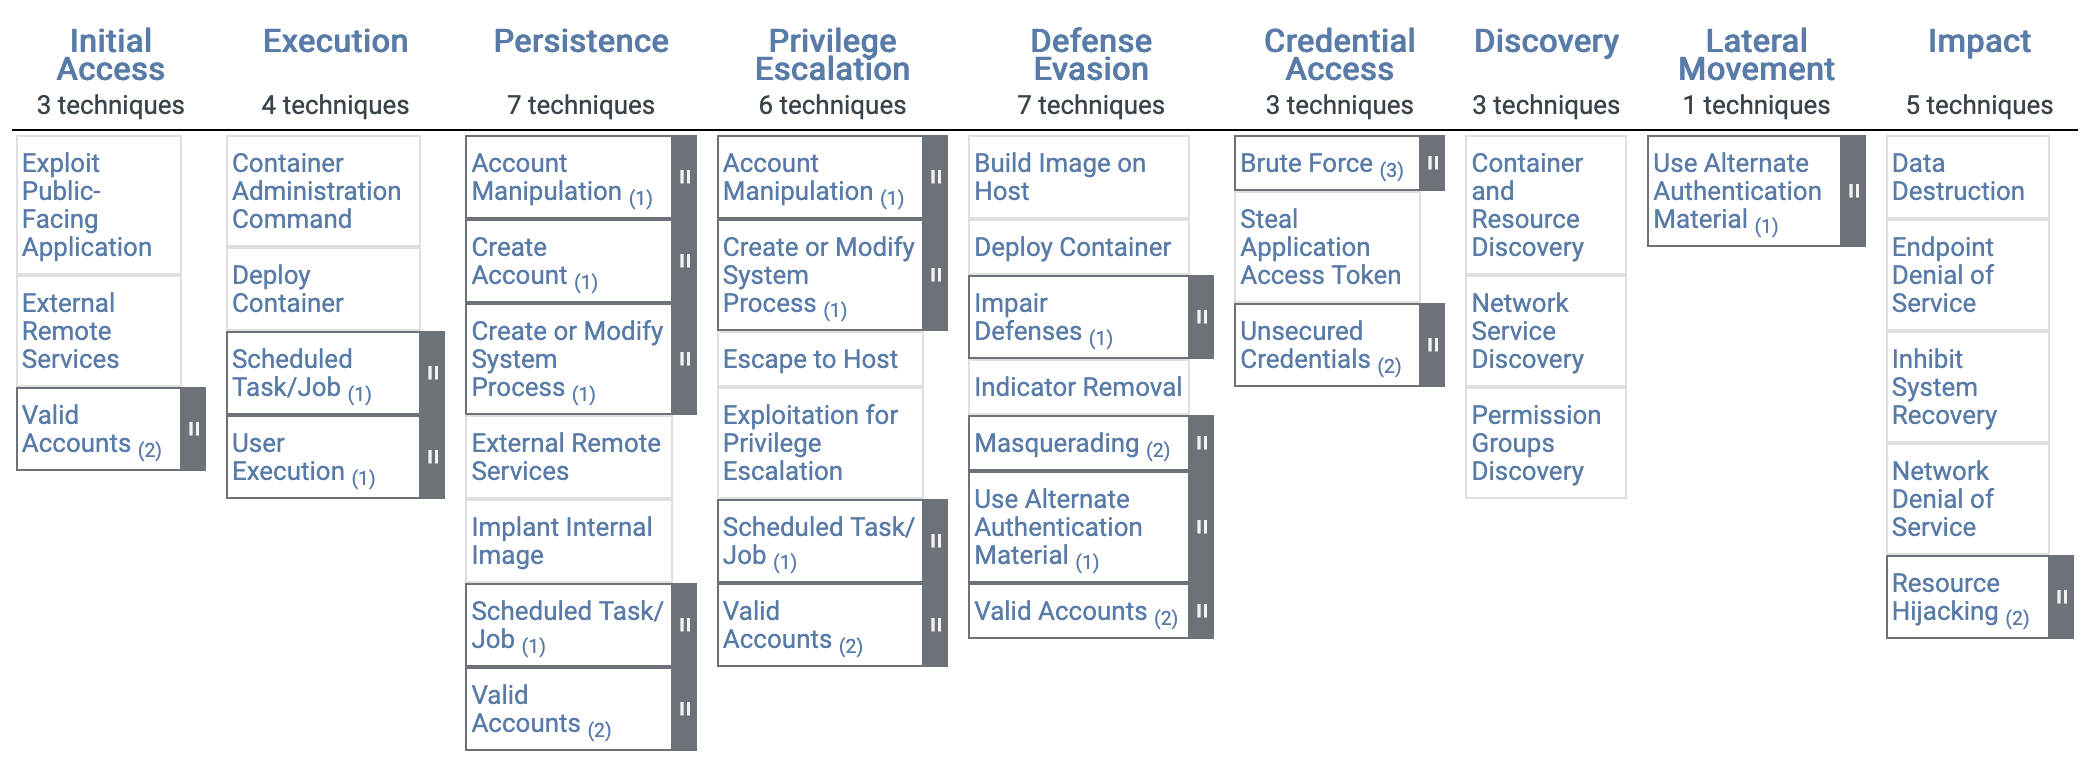
\includegraphics[width=\textwidth]{images/mitre-attack-matrix.png}
        \caption{MITRE ATT\&CK matrix for the Container platform \cite{mitre-attack-framework}.}
		\label{img:mitre-attack-matrix}
	\end{center}
\end{figure}



